\documentclass{beamer}
%\usepackage[utf8]{inputenc}

\usepackage{amsmath, amssymb}
\usepackage{zxjatype}
\usepackage[ipa]{zxjafont}
\usepackage{mymacro}

\usefonttheme{professionalfonts}
\setbeamertemplate{navigation symbols}{}

% --- page number ---
\setbeamertemplate{footline}{%
	\raisebox{10pt}{\makebox[\paperwidth]{\hfill\makebox[7em]{\normalsize\texttt{\insertframenumber/\inserttotalframenumber}}}}%
}

% Presenter's note
% \setbeameroption{show notes on second screen}

\title{Beamer Example}
\author{eqs}
\date{\today}

\begin{document}

    \begin{frame}[plain]
        \maketitle
    \end{frame}

    \begin{frame}{About this Beamer project}
        \begin{itemize}
            \item This template is available for both Japanese and English.
            \item 日本語と英語のどっちのプレゼンでも使えます.
        \end{itemize}
        \note{
            Please write presenter's note here.
            発表者ノートはここに書く.
        }
    \end{frame}

    \begin{frame}[fragile]{Commands for brackets in equations}
        \begin{itemize}
            \item \verb|\nbracket|: \verb|\left( ... \right)|
                \begin{align*}
                    \lim_{x \to \infty} \nbracket{1 + \frac{1}{x}}^x = e
                \end{align*}
            \item \verb|\cbracket|: \verb|\left\{ ... \right\}|
                \begin{align*}
                    \frac{\beta}{2}\sum_{n=1}^N \cbracket{t_n - \mathbf w^\top\boldsymbol\phi(\mathbf x_n)}^2
                \end{align*}
            \item \verb|\rbracket|: \verb|\left[ ... \right]|
            \item \verb|\abracket|: \verb|\left\langle ... \right\rangle|
        \end{itemize}
    \end{frame}

    \begin{frame}[fragile]{Highlight Commands}
        \begin{itemize}
            \item \verb|\highlight|
            \item \verb|\highlightcap|
            \item \verb|\highlightcaphead|
            \item \verb|\highlightcapoverlay|
            \item \verb|\highlightcapheadoverlay|
        \end{itemize}
    \end{frame}

    \begin{frame}[plain,c]
        \begin{center}
            \Large Example Slides
        \end{center}
    \end{frame}

    \begin{frame}{Example 1 (\texttt{highlight})}
        \begin{align*}
            &x^2 - 6x + 2 \\
            &= \highlight[red]{x^2 - 6x + 9} - 7 \\
            &= \highlight[red]{(x - 3)^2} - 7
        \end{align*}
    \end{frame}

    \begin{frame}{Example 2 (\texttt{highlightcap}, \texttt{cbracket})}
        When we consider a Gaussian prior $p(\mathbf w | \alpha) = \mathcal N(\mathbf w | \boldsymbol 0, \alpha^{-1}\mathbf I)$,
        maximization of the corresponding posterior $p(\mathbf w | \boldsf{t})$ with respect to $\mathbf w$ is equivalent to the minimization of
        \begin{align*}
            \highlightcap<2->[red]{\displaystyle\frac{\beta}{2}\sum_{n=1}^N \cbracket{t_n - \mathbf w^\top\boldsymbol\phi(\mathbf x_n)}^2}{an error function}
            + \highlightcap<3->[blue]{\displaystyle\frac{\alpha}{2}\mathbf w^\top\mathbf w}{a quadratic regularization} \tag{3.55'}
        \end{align*}
        the minimization corresponds to (3.27) with $\lambda = \alpha/\beta$.
    \end{frame}

    \begin{frame}{Example 3 (\texttt{highlightcapoverlay})}
        For the moment, the noise precision $\beta$ as a known constant.
        Where the likelihood function of $t$ is defined as:
        %%begin novalidate
        \begin{align*}
            p(\boldsf t | \mathbf w)
            = \prod_{n=1}^N
                \highlightcapoverlay<2->{\mathcal N(t_n | \mathbf w^\top \boldsymbol\phi(\mathbf x_n), \beta^{-1})}{The exponential of a quadratic func.\ of $\mathbf w$} \tag{3.10'}
        \end{align*}
        %%end novalidate
    \end{frame}

    \begin{frame}{Example 4 (multi-columns)}
        \begin{columns}[c]
            \begin{column}{0.6\hsize}\centering
                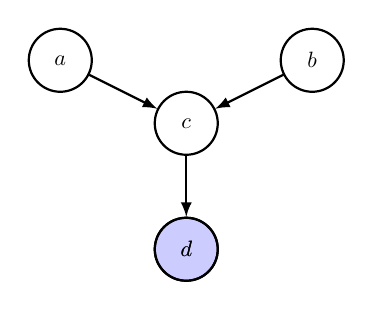
\begin{tikzpicture}[thick,scale=0.8, every node/.style={scale=0.8}]
                    \node[draw, circle, minimum width=1cm] (a) at (-2, 1) {$a$};
                    \node[draw, circle, minimum width=1cm] (c) at (0, 0) {$c$};
                    \node[draw, circle, minimum width=1cm] (b) at (2, 1) {$b$};
                    \alt<2->{
                        \node[draw, circle, minimum width=1cm, fill=blue!20!white]
                            (d) at (0, -2) {$d$};
                    }{
                        \node[draw, circle, minimum width=1cm] (d) at (0, -2) {$d$};
                    }
                    \draw[-latex] (a) -- (c);
                    \draw[-latex] (b) -- (c);
                    \draw[-latex] (c) -- (d);
                \end{tikzpicture}
            \end{column}
            \begin{column}{0.4\hsize}
                \begin{itemize}
                    \item Item 1
                    \item Item 2
                    \item Item 3
                \end{itemize}
            \end{column}
        \end{columns}
    \end{frame}
\end{document}
